% Chapter Template

\chapter{Plan Production and Management} % Main chapter title

\label{chapter-plan_management} % Change X to a consecutive number; for referencing this chapter elsewhere, use \ref{ChapterX}

\lhead{Chapter . \emph{Plan Production and Management}} % Change X to a consecutive number; this is for the header on each page - perhaps a shortened title


\section{Introduction}
\label{sec-plan_management-intro}
\subsection{Cooperation between agents}
Robots can be used to perform a large number of different operations. Some of these will be simple enough that the robot can just achieve its task by performing a prefixed sequence of elementary actions . In other cases, the robot might have to  achieve complex goals, which require the ability to create plans of actions, adapting them to the current state of the world. When cooperating together with other agents, the robot will have to build a shared plan, which includes the actions that every agent need to perform, in order to coordinate and ensure the corrent achievemt of the goal. We can imagine the following process:
\begin{itemize}
	\item The system receives a new goal. This can be directly introduced by a human, or chosen after some kind of reasoning by the robot.
	\item One of the agents (the robot or the humans) proposes a shared plan to achieve the goal, and presents it to the other agents.
	\item The agents negotiate the plan. In some situations, one of the agents might not be able (or might not want) to perform a specific action, or sequence of actions. The agent can refuse a plan, propose a correction, or propose a complete different plan.
	\item The agents execute the plan. Each agent performs its part of the plan. In additions, agents may check the state of others to monitor the correct execution of their part of the plan or too cordinate with them.
	\item An agent might fail its part of the plan. If this happens the agents need to create a new plan to account for this failure.
 	\item The process continues until the goal is achieved or it becomes inachievable (for example, a needed resource is no longer available).
\end{itemize} 
When humans cooperate this process can be very quick. For simple tasks humans are able to coordinate without explicitly forming a plan, in particular if they are used to cooperating together. Other times, when there are unexpected problems during the execution of a plan, humans are able to quickly readapt their plan, without completely restarting this process. In order to cooperate in a natural way with humans, robots need to reproduce these mechanisms.


\subsection{Multi Agent Planning}
Multi-Agent planning   is an important and studied topic in the AI community \cite{durfee1999survey}. There are several approaches to this problem, both using classical or probabilistc planning. There are several issues to consider:
\begin{itemize}
\item Localized vs Centralized: a multi-agent planner might be localized, meaning that separate systems plan independently and then communicate to build a shared plan (an idea investigated, for example in \ref{nikolaidis2013cross,guestrin2002distributed} ); or centralized, meaning that a single system plans for all the agents.
\item Coordination: agents need to coordinate their plans, in particular in the presence of shared resources. Imagine, for example, two agents, Max and Bob, that are using a tool to repair a set of cars. If Max is proceeding faster than Bob and the two don't coordinate, Max might take the tool and leave, starting to repair another car, ignoring the fact that Max still needs the tool. This example shows that it is important to reason on the duration of actions performed by agents. At the simplest level, agents need to know the advancament of the sub-plan of other agents. More complex reasoning might take into account how long an agent needs to perform a certain sub-task to refine a plan. 
\item Cooperation: even when performing different sub-tasks of the same plans, agents can help each other, for example by passing items, thus improving the optimality of the plan. Multi-Agent problems can be loosely or tightly coupled, depending on the quantity of interactions between agents. \cite{torreno2015approach} propose a general purpose approach able to plan at differet level of coupling.
\item Communication and Knowledge. In a multi-agent environment each agent might have an incomplete or incorrent belief on the world, which might lead to wrong or suboptimal actions. Agents may communicate to progressively build a correct belief model on the state world. 
\end{itemize}


Several approaches has been studied to bring the multi-agent planning problem in a probabilistic framework. \cite{boutilier1999sequential} create a centralized MDP, able to select at each time step actions for every present agent. Dec-POMDP \cite{bernstein2002complexity} and I-POMDP \cite{gmytrasiewicz2005framework} are more complex frameworks, that take into account the belief models of agents. Both models are much more complex than normal MDP\POMDPs, and result difficult to use in even moderately complex scenarios. A solution to this problem is considering simpler problem, where the agents mostly work independently and interact only in limited situations, such as in \cite{molo2013heuristic}. 

\subsection{Plan Explanation and Negotiation}
In order to form a shared plans, agents often communicate, explaining tasks to each other and negotiating to agree on a solution. In \cite{Lallee2013} the authors suggest that joint plans should be fully communicated in order to sustain effective collaboration. 

Some authors have started to investigate this topic in robotics. In \cite{Petit2012}, a human is able to teach new plans to a robot verbally through ``spoken language programming''. \cite{Sorce2015} studies the inverse problem, where the system is able to explain plans to users. 

%negotiation
fabregues2014hana

\subsection{Plan Management}
Finally, the shared plan needs to be executed. Agents need to perform their part of the plans and to monitor other agents in order to coordinate with them. Two examples of systems able to execute shared plans are  \cite{shah2011improved} and Pike \cite{karpas2015robust}. Chaski is also able to execute plans in two different modalities: equal partners or leader and assistent.



\section{Overview}
\label{sec-plan_management-overview}
Our system presents a planning layer which is able to perform the following tasks:
\begin{itemize}
	\item Interface with external planners in order to create a shared plan. The system has been integrated with an HTN (Hierarchical Task Network) based planner, HATP (Human-Aware Task Planner) , and with a multi-agent MDP planner.
	\item Explain a plan to human agents. Depending on the human knowledge of the tasks to be performed, the robot will change the explanations, explaining more deeply tasks that agents don't know. This idea is supported by research on Intelligent Tutoring Systems \cite{brusilovskiy1994construction}  and on e-learning \cite{brusilovskiy2005}, which  prove the necessity of keeping and updating a model of the learner's knowledge to efficiently teach a task.
	\item Negotiate a plan. Our system has some simple mechanics allowing a human to reject a plan, specifying which parts of it it does not want to perform. The robot will take the human's preference into account when producing a new plan.
	\item Monitor a human plan. Our system is able to monitor other agents' parts of a plan, too cordinate with them and to react when the an agent fails an action or his action diverge from the current plan.
	\item Receive plans from a user. Users can interact with the robot with a tablet application, asking it to execute specific actions or goals.
	\item Executing shared plans in different modalities. The robot can be a leader, assistant, or equal partner of humans during plan management.
\end{itemize}

A number of modules implement this ideas, as shown in figure \ref{fig:plan_management-architecture}:
\begin{itemize}
\item Task Planner. Creates a shared plan for the involved agents.
\item Plan Explanation. Explains the plan to the involved agents, adapting it to their knowledge.
\item Plan Negotiation. Negotiats the plan with the involved agents.
\item Plan Management. Manages the current plan, interacting with the Plan Execution layer to execute the robot's action and with the Situation Assessment layer to monitor human's actions.
\end{itemize}

After receiving a goal from the Goal Management layer, the Task Planner looks for a suitable plan. If there is a plan, depending from the current modality, it will activate Plan Explanation and the Plan Negotiation modules to communicate with the involved humans, or directly send the plan to the Plan Management module. If the plan needs to be negotiated this process is repeated. When a plan is agreed by all the agents, the Task Planner sends it to the Plan Management module, which executes it. 

\begin{figure}[h!]
	\centering
	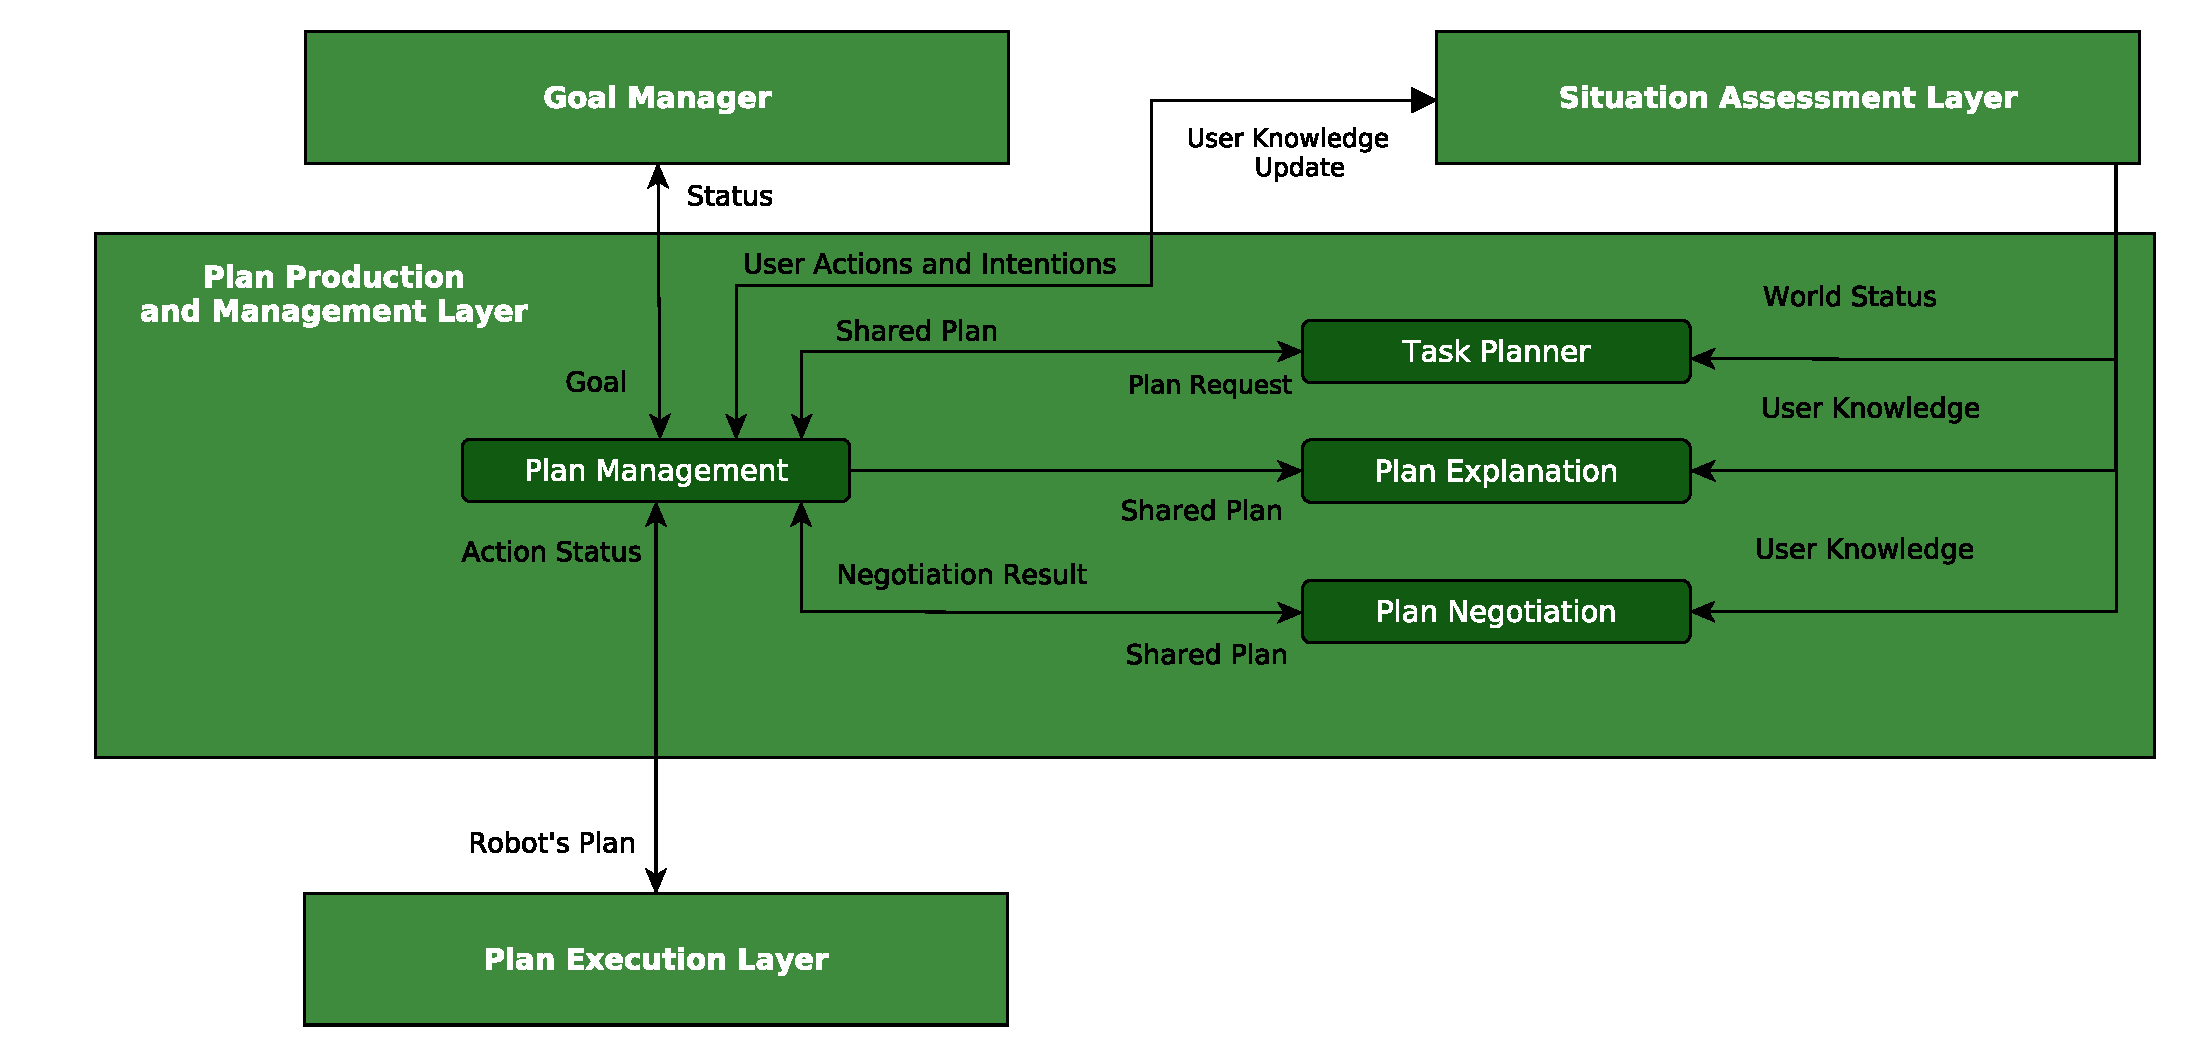
\includegraphics[clip,scale=0.6]{img/plan_management/architecture.pdf}
	\caption{The image represents the architecture of the plan management layers. Yellow rounded rectangles represent modules, while blue rectangles layers. Arrows represent message exchanged between components, with the label detailing the message. }
	\label{fig:goal_management-goal_cycle}
\end{figure}


Part of this chapter was presented in \cite{Lallement2014,milliez2016using,fioreiser2014}.

\section{Plan Management Modalities}
\label{sec-plan_management-modalities}
When acting together, agents sometimes do not have the same decision power, with one of them assuming the role of a leader. We represent this idea, in our system, by proposing three different modalities: Robot Leader, Human Leader, and Equal Partners. The robot is able to switch from one modality to another during the execution of a plan. For example, if the current modality is 'Robot Leader' and the Robot receives a command from a user, it will switch to the 'Human Leader' modality, after interrupting its current action.

\subsection{Robot Leader}
In this modality the robot, after computing the plan, will explain it, negotiate it and start executing it.
The robot will track the status of humans, informing them of which actions they should execute. This modality can be helpful when interacting with  naive users or in tasks where the robot has a better knowledge of the
domain or of the environment than the other agents.

\subsection{Human Leader}
The human can also create plans, interacting with the robot by using a
tablet application, as explained in chapter \ref{sec:situation_assessment-communication}. In this modality the robot   will simply observe the surroundings and wait for user inputs. This modality is always available and has a priority over
the other two modalities. If the robot receives a command from the
application while it is in another modality, it will abandon its current
plan, stopping its actions at a safe point, and then execute the users'
command. We feel that this interaction modality is important for two
different reasons.  First, some users will simply prefer to be in
charge of the execution process, for a matter of personal preference or because they
feel they have a deeper knowledge on how to realize the current task
than the robot. We can picture, for example, industrial or medical
scenarios, where the human is the leader and asks the robot to perform
different tasks to help him, when needed. A second use of this modality is in situations where
the robot doesn't have  a clear estimation of the users' intentions and
goals. For example, in a domestic environment, a user could decide to
order a robot to bring him a drink, a need that the robot can't always anticipate.

\subsection{Equal Partners}
In the last presented operation modality the robot will try to help
the human to complete a task. At the start of the scenario, the robot
will stand still and observe the environment. After the user takes an
action the robot will calculate a plan and try to help as it can, by
performing actions related to that task and by giving helpful information to
the user, for example to fill gaps in their knowledge. In this modality, 
the robot will not explain or negotiate the current plan.

We feel that, particularly in non-critical tasks, where defining an accurate plan between the partners is not
fundamental, this modality is a very natural way of
interaction between different partners.

\section{Human Knowledge and Plan Management}
\label{sec-plan_management-human_knowledge}
\subsection{Representing Human Knowledge in a Task}
Among the topics of this chapter, we will consider different ways to use human knowledge in planning issues. In order to do so, we introduce and maintain, a new property of human knowledge of a task, which will be maintained in the Situation Assessment Layer. 

This property is represented as a tuple $(human, task, parameters, value)$, where $human$ is a string identifying the subject of this property, $task$ is the name of the related task, $parameters$ is a list of relevant parameters used to describe knowledge in the task, and $value$ is the level of knowledge in the task. Knowledge values can be assigned from the set $[new, beginner, intermediate, expert]$.  For example, we can represent the fact that Bob knows very well how to fix a wheel to a car with the tuple $(Bob, fix_wheel, car, expert)$. 

Parameters can be deeply linked to the knowledge of a task. In general, we can divide task parameters in two categories:
\begin{itemize}
\item class-link. In some situation, knowledge of a task is not linked to the specific instance of a parameter, but to a whole class. For example, we can imagine that if Bob knows how to paint the living room, he will know how to paint every room in a standard house. We could represent this property as $(Bob, paint, house_room, expert)$. We can notice that the parameter, in this case, is $house_room$, representing the class of rooms belonging to a normal house, and not $living_room$.
\item instance-link. In other cases, instead, knowledge of a task is deeply linked to specific instances of parameters. For example, knowing how to fix the motor of a specific car, wouldn't necessary translate in knowing how to fix the motor of every car.
\end{itemize}

We can also consider some tasks as common knowledge, expecting every human to be able to perform them, like, for example, putting ingredients in a bowl. of task will be tagged as common knowledge and considered as known by any user, no matter the parameters. 

\subsection{Maintaning Human Knowledge in a Task}
%How human update their knowledge
We define four task-knowledge levels for humans, that will lead to different behaviors from the robot.

\begin{itemize}
\item \textit{New}.this value will be used for tasks which have never been performed by the user. If the user observes the task being executed, with an explanation of it, or if he performs it himself, the value will be changed to \textit{beginner}. However if the user observes the task being executed without any explanation, we  keep the level as \textit{new} since we consider that he might not have received enough information to link the observed movements to the task.
\item \textit{beginner}. This value will be used for users who have already achieved the task but may still need explanation to perform it again. If the user successfully performs the task again, without asking for explanations, the value is changed to \textit{intermediate}, otherwise it is changed to \textit{new}.
\item \textit{Intermediate}. This value will be used for users who are able to perform the task without guidance. If the user successfully performs the task without guidance again, the value is changed to \textit{expert}. In case of failure, it is downgraded to \textit{beginner}.
\item \textit{Expert}. This knowledge level will be used for users who are able to perform the task without guidance and are experienced enough to explain it to a third party. If the user fails in performing the task, he will be downgraded to \textit{intermediate}.
\end{itemize}

These task knowledge levels allow for adaptation of the collaborative plan generation, explanation and monitoring.


\section{Plan Generation}
\label{sec-plan_management-plan_generation}
\subsection{Introduction}
\label{subsec-plan_management_hatp}
One of the goals of our system is flexibility; we consider important important the possibility to interface with external components. We built an intermediate Plan Generation module, that interacts with external planners and returns plans represented in a common format that can be handled by other modules. At the moment, we tested two different planners with our system, which will be shown in the next subsections.

\subsection{Human-Aware Task Planner}
Computing a plan in complex environments can be very complex and time consuming. An useful approach to reduce planning's search space is introducing the knowledge of an expert in the planner, in order to guide it to desiderable states. An implementation of this idea is HTN, where the domain expert specifies a hierarchical library of operations, called tasks and actions, when the operation is respectively a node or a leaf in the hierarchy.  HATP is a planning framework that extends HTN for human-robot interaction tasks. Among the capacities of HATP we can find:
\begin{itemize}
\item Multi-Agent. HATP is able to plan for different agents at the same time, humans and robots.
\item Social Rules. The domain expert can introduce a set of rules, which represent desirable behaviors, for example to distribute in different ways operations between agents, or to avoid specific sequences of actions.
\item Cost Driven. The domain expert can specify a cost for actions. Plan pruning allows to explore more efficiently the search space, discarding paths that are not promising.
\end{itemize} 

Plans are represented as an HTN tree decomposition and as a set of streams, one per agent, which shows which actions each agent needs to perform. Casual links are introduced between streams to ensure synchronization.

\subsection{Human-Aware Probabilistic Planner}
\label{subsec-plan_management_happ}

% dietterich2000hierarchical
% This paper presents a new approach to hierarchical reinforcement learning based on de-
% composing the target Markov decision process (MDP) into a hierarchy of smaller MDPs
% and decomposing the value function of the target MDP into an additive combination of the value functions of the smaller MDPs. The decomposition, known as the MAXQ decom-position, has both a procedural semantics|as a subroutine hierarchy|and a declarative
% semantics|as a representation of the value function of a hierarchical policy. MAXQ uni
% and extends previous work on hierarchical reinforcement learning by Singh, Kaelbling, and
% Dayan and Hinton. It is based on the assumption that the programmer can identify useful
% subgoals and de
% programmer constrains the set of policies that need to be considered during reinforcement
% learning. The MAXQ value function decomposition can represent the value function of any
% policy that is consistent with the given hierarchy. The decomposition also creates oppor-
% tunities to exploit state abstractions, so that individual MDPs within the hierarchy can
% ignore large parts of the state space


% hauskrecht1998hierarchical
% We investigate the use of temporally abstract
% actions, or macro-actions, in the solution of
% Markov decision processes. Unlike current mod-
% els that combine both primitive actions and
% macro-actions and leave the state space un-
% changed, we propose a hierarchical model (using
% an abstract MDP) that works with macro-actions
% only, and that significantly reduces the size of the
% state space. This is achieved by treating macro-
% actions as local policies that act in certain regions
% of state space, and by restricting states in the ab-
% stract MDP to those at the boundaries of regions.
% The abstract MDP approximates the original and
% can be solved more efficiently. We discuss sev-
% eral ways in which macro-actions can be gen-
% erated to ensure good solution quality. Finally,
% we consider ways in which macro-actions can be
% reused to solve multiple, related MDPs; and we
% show that this can justify the computational over-
% head of macro-action generation.


\subsection{Adapting Plan Generation to Human Knowledge}
\label{subsec-plan_generation-adapting_knowledge}
When interacting with humans, it is important to take into account others' knowledge and capacities when planning. We consider two different policies for our planner: teaching, where the planner will look for plans not known to the human, in order to teach him of different ways of achieving a task; and efficiency, where the robot will try to maximize the number of human tasks known when creating a plan. This ideas where represented as social rules.

To illustrate our planner and the new social rule let us consider the toy example where a human and a robot have to cook an apple pie. A part of the solution plan is shown in Figure \ref{fig:plan_management-treePlan}. In this context we can consider that the human knows how to carry out all the actions (pick, place, cut, and so on) but he might not know the correct sequence to achieve the goal. If we favor teaching, the plan should contain a way to achieve the recipe with a minimal knowledge level on each task and, as much as possible, the human should be in charge of those steps. On the other hand, if we favor efficiency the plan should contain the smallest amount of unknown tasks to be performed by the user.
Using this rule, the robot is able to adapt its plan generation to the knowledge of the user concerning tasks contained in the shared plan.

To properly compute the cost of a plan, the planner will also consider a task knowledge as upgraded once it is added to the plan. This allows the efficiency policy to prefer plans that reuse the same task many times and assign it to the same user to lower the cost, over some plans where different tasks are performed or the same task is performed by a different agent.

The planner is integrated in a dialog system that allows to negotiate plans, as explained in \ref{sec:plan_management-negotiation}. Using this system, the preference and abilities of users are recorded in the Situation Assessment Layer. 
If a user is not able to perform a certain task, the planner will never chose this action for him. If he user prefers to perform, or not to perform, a specific task, the planner will update the cost functions accordingly with a reward or penality to assign that task to that user.

\section{Plan Explanation}
\label{sec:plan_management-plan_explanation}
Once the system has genereated a collaborative plan, this must be shared with the human partners. The robot will present and negotiate plans using speech, which is supported by several studies, such as \cite{Lalle2013,tomasello2005}.

\subsection{Plan Preprocessing}
The structured tree generated by the planner represents a solution to achieve the goal. In order to explain this plan to users, the system will process it, removing unnecessary information. In particular, our algorithm follows two rules:
\begin{itemize}
	\item  We remove recursive tasks. If a node $n$ of the HTN tree contains the same method as its parent $parent(n)$, it will be replaced in the tree by its children $children(n)$. 
	\item We replace nodes with a single child by their children.
\end{itemize}

More formally:
\begin{enumerate}
\item $\textbf{if}$ $(compare(n, parent(n)))$ \textbf{then} $n \leftarrow children(n)$
\item $\textbf{if}$ $(children(n).size() = 1)$ \textbf{then} $n \leftarrow children(n)$
\end{enumerate}

where $compare(n1,n2)$ is true if the two nodes have the same method.

\subsection{Plan Presentation}
Before executing the plan, the robot will present the goal and the proposed allocation of high-level tasks to give a global view on the plan. Standard natural language generation is used as shown in Table \ref{table:plan_management-pie-present}. 
To ensure the scalability of the system, when presenting the plan, the robot will verbalize only the $N$ first highest level tasks. For simplicity, we have chosen $N$=$3$ based on some runs carried out during the development process. We believe that this number would require further investigation depending on the domain or on the user and his confidence in the execution of the tasks. The robot will present the first steps of the plan, and then execute them. Once these steps have been executed, the robot will repeat the present/negotiate/execute process until the plan is completed or aborted.

% Put in a double colomn table
%\begin{tabular}{ll}
%   agents(root) $+$ have\_to $+$ root  & "We have to cook an apple pie." \\
%   introduce\_presentation & "I will tell you the steps." \\
%   agents(root.child[0]) $+$ first $+$ root.child[0] & "You will first fetch the ingredients," \\
%   then $+$ agents(root.child[1]) $+$  root.child[1] & "Then I will assemble the apple pie," \\
%   finally $+$ agents(root.child[2]) $+$  root.child[2] & "Finally you will bake the apple pie in the oven." \\


%\end{tabular}
 
 
 \begin{table}
 %\vspace{-10pt}
\centering
\scriptsize
\renewcommand{\arraystretch}{1.3}
\begin{tabular}{c|c}
   agents(root) $+$ have\_to $+$ root  & "We have to cook an apple pie." \\
   \hline
   introduce\_presentation & "I will tell you the steps." \\
   \hline
   agents(child[0]) $+$ first $+$ child[0] & "You will first fetch the ingredients," \\
   \hline
   then $+$ agents(child[1]) $+$  child[1] & "Then I will assemble the apple pie," \\
   \hline
   finally $+$ agents(child[2]) $+$  child[2] & "Finally, you will bake \\
   & the apple pie in the oven." \\
\end{tabular}
 \vspace{-4pt}
\caption{Presentation of a plan to cook an apple pie. Root is the root of the tree and child is a list with its children.}
 \vspace{-20pt}
 \label{table:plan_management-pie-present}    
\end{table}

\section{Plan Negotiation}
\label{plan_managemet-plan_negotiation}
Once the robot has presented the plan it generated to achieve the joint goal to his collaborators, the robot can start a negotiation phase. 

We introduce a simple negotiation algorithm, that starts with the robot asking humans for approval, inquiring what is wrong in case of disagreement. We handle two different human requests. First, the user can express his preferences, either to perform a task previously assigned to the robot or the not perform a task assigned to him. The other possibility is to inform the robot that the user cannot perform an action. The system will store these information and try to find a new plan, taking them into account, before starting a new explanation and negotiation phase.
 
\section{Plan Management}
\label{sec:plan_management-planExecution}

Once the plan has been accepted by the collaborator, the agents can start executing it. While executing its part of the plan, by interacting with the Plan Execution Layer, the robot will choose which tasks to explain to users, and which tasks to monitor. We present our plan management algorithm, which will then be explained.


\section{Plan Monitoring}
\subsection{Introduction}
During the execution of a plan, the robot will monitor other agents. In general, having a shared plan, the robot knows what is the user's next expected action, and can monitor if it's accomplished. Plan monitoring poses a number of different issues:
\begin{itemize}
\item Understanding when the next expected action has been performed. In some situations the robot will monitor the execution of a specific action. In this event, it needs to understand when the action has been performed.
\item Understanding when the next expected task has been performed. In some situations, the robot wants to give a human cooperator the freedom to perform a subtask has it sees fit. This is a more complex problem than monitoring a specific action, since the robot needs to reason on the results of sequences of actions.
\item Evaluating the human engagement in the current task. The robot needs to understand if the human is trying to accomplish its current task, if he momentarily interrupted it, or if he abandoned it.
\end{itemize}

\subsection{Monitoring Plans}
When executing a shared goal, the Plan Management Layer needs to interact with the Intention and Actions recognition module in the Situation Assessment Layer. Normally, this module only monitors single goals. This is not enough when actively cooperating in a joint task, since actions may vary if the load of the task is shared. While performing a shared plan, we create a new intention for each node in the plan tree that can be currently performed (meaning, if it has conditional links to other nodes, they have already been accomplished). We associate to these intentions the linked MMDP, as previously explained in \ref{subsec:plan_management-happ}, and the context node "have a shared plan", which is treated as evidence with the value true. We call these intentions $plan intentions$.

We associate to each known intention a precomputed "expected length", which is the time to accomplish the linked goal.

The robot can be updated at each time on what actions have been performed, using the mechanisms described in Section \ref{sec:situation_assesssment-intention_recognition}. This way, the robot can compare the actions performed by humans, with those that should be performed following the shared plan.

Using the Intention and Action Recognition module, the robot can infer in which intention the human is currently involved. If the current involved intention equals the task to monitor, the robot infers that the human is actively working to complete it's task. The task will be completed when the linked MMDP reaches a goal state, and at that point the monitor procedure will return a success.

If the human is currently not involved in the monitored task there are three possibilities:
\begin{itemize}
	\item the human has momentarily interrupted the task. This can be inferred if the human is currently involved in another intention, which doesn't belong to the $plan intentions$, and who's expected length is short. In this case, the monitor won't return an error until a predefined $allowed_time$.
	\item the human has abandoned the task.  This can be inferred if the human is currently involved in another intention, which doesn't belong to the $plan intentions$, and who's expected length is long. The monitor will return a "not involved error". 
	\item the human is performing another task in the shared goal. This can be inferred if the human is currently involved in another intention, which belongs to the $plan intentions$. In this case the monitor will return a "other task error"
\end{itemize}


\subsection{Monitoring and Unseen Actions}
Often, in cooperative tasks, the agents will operate in different locations, and so their actions won't be observable at all time. Perhaps one of the agents is preparing a cake in the kitchen,  while the robot is preparing the table. While we don't deal, in this work, with these issues, there are studies on plan recognition in partially observable environments, like \cite{geib2005partial}.



\subsection{Failed Monitoring and Replanning}
What happens when a human is not engaged in the current task? There are three possibilities:
\begin{itemize}
\item The human is momentarily doing another task: in this case, the robot will simply wait, without considering the human's assigned task as failed.
\item The human is engaged in a different long-term task, related to the current scenario: in this case, the robot will act differently depending on the current modality. In the 'robot leader' mode, the monitoring will be considered as failure. In the 'Equal Partners' or 'Human Leader' modalities, the robot will create a new plan, and try to adapt to the human.  
\item The human is engaged in a different long-term task, not related to the current scenario. In this case, the monitor will return a failure.
\end{itemize}

To understand if a task is 'short term' or 'long term' we can hand-code these information, linking it to the intentions. We infer that a human is engaged in a different task, but still related to the same scenario, if the likelihood that the human intention is its assigned task is low, but the likelihood that the human intention is the shared goal is still high. 



\section{Experiments and Discussion}
\label{study}

\subsection{User Study}
We have conducted a comparative user study in order to have a first evaluation of the perception by users of our system's adaptability. Two groups of users were asked to follow the two-pies scenario. The first group interacted with a simulated robot equipped with a basic system (BS). BS has the same behavior as our system without the agent knowledge awareness mechanisms. The second group interacted with a second system, called knowledge system (KS), showing a behavior similar to what our system provides.
All participants were then asked to evaluate the interaction with respect to several criteria.
%
The task distribution presented in Section \ref{sec:experiment} 
is used for both systems to achieve the apple pie cooking example.
Once they have cooked the first dessert, the robot generates a plan to cook the banana pie. 
In KS,  the robot has the same behavior as our system and  favors a task distribution for the banana pie where the human performs tasks he has already performed for the apple pie (preparing dough and fruits).
In BS, we imagine that the robot could ask the human to make the mixture instead of the dough.

Two groups of 19 participants, from 18 to 60, interacted with each system. This was achieved thanks to  
an online user study\footnote{User study for KS http://goo.gl/forms/qvbtu4vcFW, and BS http://goo.gl/forms/ZSvGcCi5le}, where we presented pictures of the task state and recordings of the robot's speech in French for each step of the interaction (as shown in Figure \ref{fig:user_study}).
On some steps, the user could choose the action to perform, making it possible to execute a wrong action leading to a replan from the robot. For simplicity, the replan was limited to cancel the wrong action before resuming the previous plan. Also, to focus on the adaptability of our solution from knowledge awareness in the different steps of the shared plan, we did not allow negotiation from the users.
At the end of the simulated interaction, we have asked the same questions to both groups, concerning the adaptability of the system and the robot partner itself. 
The users gave marks along a Likert scale from one (disagree) to five (agree) to express their agreement with several statements (as shown in Figure \ref{fig:user_study}).
For instance, one question we asked: "Did you feel that the robot adapts its explanation to the knowledge you acquired during the interaction?".

\begin{figure}[ht!]
  \vspace{-8pt}
 \centering
 \begin{tabular}{cc}
  \includegraphics[width=0.24\textwidth]{img/ustudy9.png} &
  \includegraphics[width=0.19\textwidth]{img/ustudy11.png}
 \end{tabular}
  \vspace{-6pt}
 \caption{\textit{Left}: The user listens to recorded robot explanation and chooses the action to take. \textit{Right}: At the end, the user evaluates the interaction using a Likert scale.}
 \label{fig:user_study}
   \vspace{-15pt}
 \end{figure}

\subsection{Results}

We collected the answers for each form, and computed the mean along with the standard deviation and p-value to evaluate the reliability. The p-value was computed using a t-distribution with 18 degrees of freedom and considering that the mean of KS would be higher than BS as stated in our hypothesis and identical as null hypothesis. 
%We compare below the results for each system. 
Figure \ref{fig:results} summarizes the results. Comparing users' answers, we can see that the robot adaptation on users' knowledge concerning the explanation is well perceived with a mean of 3.74 for KS against 2.05 for BS. The users interacting with KS globally noticed that the task distribution took their knowledge into account by giving a mean rating of 3.42 for KS and 2.58 for BS. The last question concerned the freedom to choose the way to perform the task. The mean was 2.58 for KS compared to 1.89 for BS, and the p-value was lower than 0.05. So even on that aspect there was an improvement. 
%As some users just performed the task as the robot teach them, they may not have noticed that they could perform it in a different way. However, 
With KS, the users attributed a mean of 3.11 for the global adaptability of the system against 1.89 for the basic one.
We also asked how the robot partner was perceived. While in BS, the robot is not perceived as more verbose (2.53 for KS against 2.47 for BS), people found the interaction slightly more natural (2.74 against 2.42) and the robot appeared smarter (2.79 against 2.26). Even if these results strengthen our idea, as the p-value is higher than 0.1 for the naturalness, it doesn't prove that there is a noticeable difference between the two systems. We believe that other aspects might have been taken into account by the users such as the speech itself and lead users of both experiments to perceive the interaction as not so natural. For instance, improving the verbalization with a synonym dictionary could help to get more significant results.



 \begin{figure}[ht!]

   \vspace{-9pt}
 \centering
 \begin{tabular}{cc}
  \includegraphics[width=0.41\textwidth]{img/respvalue3.png}
 \end{tabular}
   \vspace{-8pt}
 \caption{Average users' rating of the interaction on several criteria. Blue for our system and red for basic system.}
 \label{fig:results}
  \vspace{-10pt}
 \end{figure}

This study sheds light on how users were able to perceive the robot adaptation to their knowledge concerning task distribution, task explanation and monitoring. In addition, the robot partner was perceived as smarter and the interaction seemed a bit more natural to the users. However these first results need to be confirmed with study on a larger population. Also, as future work we envisage to conduct this users study on a real robot as we believe it would lead to more realistic opinions.
In both studies, we asked the participants how the interaction could be improved. Several users suggested they would like to be able to choose which action to perform, putting forward the importance of the negotiation (we removed negotiation in the user study to focus on knowledge adaptation). A user suggested they would like to be informed about the progress from time to time. This can be easily added since at each moment the robot knows the number of nodes remaining in the shared plan to achieve the goal.
Other comments concerned suggestions about the speech itself, the robot voice, intonation and chosen words, which were not the aim of the experiment but are indeed an important part of the interaction. 

%


